\chapter{State of the art: Data collection and Techniques for Authorship Attribution}

%%Description of the training iperparameters (CODE IN APPENDIX)
Word2vec (Mikolov et al., 2013a) has gained kinds of traction today. As the name shows, it translates words to vectors called word embeddings. That is to say, it gets the vector representations of words. We used gensim\footnote{\url{https://radimrehurek.com/gensim/}}, a python tool, to get word2vec module, that uses by default Continuos Bag of Words (CBOW) method.

\section{SVM studies}

\subsection{SVM studies on authorship attribution}

\section{GDELT studies}

\subsection{Victorian era books}

\subsection{Authorship attribution GDELT}

\section{RCV1 studies}

\subsection{Studies on RCV1 on authorship attribution}

\section{The guardian studies}

\subsection{Cross-topic authorship attribution}

\section{Studies on Stanford Amazon Food Reviews}

\section{Dataset selection}


The elements that have an impact on the performance of the model are the input corpora, model architecture and the hyper-parameters.
In many works lemmatized, lowercased and shuffled input during training the word2vec are recommended; we carried out our experiments with these settings as detailed above.\\
For each corpus we used different approach for the documents vocabulary of the training model, such as:
\begin{itemize}
	\item \textbf{ICD-9-CM Dictionary:} we used every entry of the dictionary as a single document
	\item \textbf{Wikipedia:} we used the entire content of each page as a single document
	\item \textbf{SDO:} we used every different diagnosis as a single document
\end{itemize}

We then made use of \textit{gensim.utils.simple\_preprocess}\footnote{\url{https://radimrehurek.com/gensim/utils.html}}, which convert a document into a list of lowercase tokens, ignoring tokens that are too short or too long.
In the end we trained each corpus separately forming 3 separate models and one joining all the documents of each corpus. Every model has been trained with the same hyperparameters:
\begin{itemize}
	\item min\_count=2 \\
	Ignores all words with total frequency lower than this.
	\item size=200 \\
	Dimensionality of the word vectors.
	\item window=10\\
	Maximum distance between the current and predicted word within a sentence.
	\item workers=10 \\
	Use these many worker threads to train the model (=faster training with multicore machines).
	\item epochs=10 \\
	Number of iterations (epochs) over the corpus.
\end{itemize}

Code for training the models can be found in Appendix \ref{appendix:trainModel}.


%During diagnosis the doctor does a lot of typing errors, with SDO I can take them in consideration

If you parse emergency room discharge records data, you can easily notice how much noisy the data are. Especially dealing with such short sentence, it's very important to take action with misspelled words. 
Table \ref{tab:tableTypingErrors} shows the first five diagnosis with at least a typo error beginning with the letter \enquote{a}. \\

\begin{table}[h!]
	\begin{center}  
		\caption[First 5 diagnosis that contains at least one typo error beginning with the letter \enquote{a}]{First 5 diagnosis in the emergency room discharge records corpus that contains at least one typo error beginning with the letter \enquote{a}.} 
		\label{tab:tableTypingErrors}
		%\resizebox{\linewidth}{!}{  %
		\begin{tabular}{|p{\linewidth}|} 
			%\toprule
			%\textbf{Diagnosis} \\
			%\midrule
			\hline
			trauma cranico non commotivo vasta flc del cuoio capelluto ferite escoriate multiple \textbf{aa} inferiori e superiori colpo di frusta del rachide cervicale	\\ \hline
			contusione aavampiede destro	\\ \hline
			frattura plurima ossa dorsali del naso con ferita lc piramide nasale contusione mano ginocchio dx \textbf{aabrasioni}	\\ \hline
			edema \textbf{aal} volto da probaile reazione allergica a ketoprofene oki	\\ \hline
			ferita profonda lacero contusa \textbf{aalla} base del dito mano ds	\\ \hline \hline
			non-committal head injury extensive wound lacerated-bruised scalp multiple excoriate wounds \textbf{ls} upper and lower whiplash of the cervical spine	\\ \hline
			right \textbf{forefooot} bruise	\\ \hline
			multiple fracture of the dorsal bones of the nose with wound tear bruised pyramid nasal bruise hand right knee \textbf{aabrasions}	\\ \hline
			edema \textbf{iin} the face from probable allergic reaction to anti-inflammatory medicine \\ \hline
			wound deep lacerated and bruised \textbf{aat} the base of the right hand finger	\\ \hline
			%\bottomrule 
		\end{tabular} 
		%}
	\end{center}
\end{table}

Word embeddings is generally a more powerful tool than to do auto-correction of misspelled words, but with our models we can do this as well.
For example in Table \ref{tab:tableTypoMostSimilar}, we can look for the most similar words to this italian misspelled words that we found in diagnosis: \textit{emoragia} (typo of bleeding) and \textit{ati} (typo of limbs). \\
The reader has to understand that our model is unsupervised, when we will show closest word vectors to the given word it will be a result solely based on the context taken from the training dataset.
In bold we point out the correct spelled corresponding word in italian.\\

\begin{table}[h!]
	\begin{center}
		\caption[Most-similar words to: \textit{emoragia} (typo of bleeding) and \textit{ati} (typo of limbs)]{Most-similar words to: \textit{emoragia} (typo of bleeding) and \textit{ati} (typo of limbs).}
		\label{tab:tableTypoMostSimilar}
		%\resizebox{\linewidth}{!}{  %
		\begin{tabular}{l|S|l|S}
			\toprule
			\textbf{emoragia} & \textbf{Value} & \textbf{ati} & \textbf{Value} \\
			\midrule
			emorraggia & 0.7617026567459106 & \textbf{arti} & 0.6036288738250732 \\
			\textbf{emorragia} & 0.7511980533599854 & tvparti & 0.5718222856521606 \\
			egdsemorragia & 0.712714433670044 & rti & 0.5638812780380249 \\
			emorrazgia & 0.6999548673629761 & artitrauma & 0.5611196756362915 \\			
			cureemorragia	& 0.6337481737136841 & artie & 0.5547841191291809 \\
			\bottomrule
		\end{tabular}
		%}
	\end{center}
\end{table}

We can also point out that correct-spelled words are less common than misspelled words for the example taken in consideration. In 
Using PCA\footnote{Principal component analysis - is a dimension-reduction tool that can be used to	reduce a large set of variables to a small set that still contains most of the information in the large set.} we can see in Figure \ref{fig:diabeteJoinData} the 2D representation of the top 10 most similar word vectors to the correct spelled italian word for diabetes. [See \ref{appendix:plotModel} for code].\\
The first 10 most similar word vectors to \textit{diabete} (diabetes) are indeed misspelled words of itself.

\begin{figure}[ht]
	\centering
	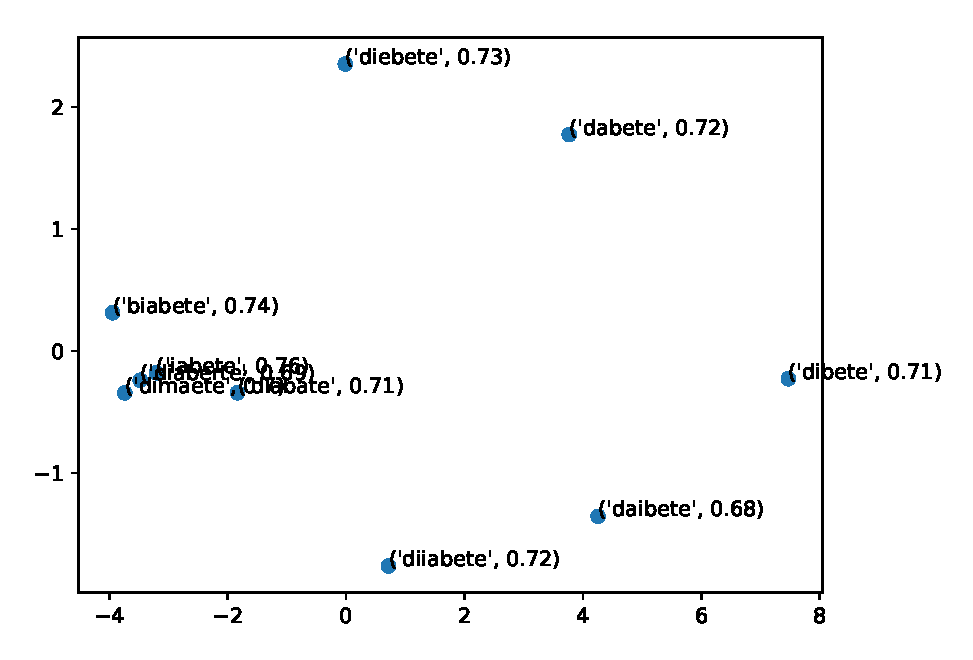
\includegraphics[width=.7\textwidth, height=.5\textheight, keepaspectratio]{diabeteJoinData}
	\caption[Diabetes - 10 most similar words plotted for JoinData model]{Top 10 most similar words to diabetes in the JoinData model.}
	\label{fig:diabeteJoinData}
\end{figure}

%Abbreviazioni non intuitive (dx, rx, tc, pz)
Medical terminology is made up of numerous Greek and/or Latin suffixes and prefixes. It describes body parts, functions, surgical procedures, and is used in medical reports. Every language has his own lingo and even every specific group of doctors has its own. When writing down an emergency room discharge records, doctors very often use abbreviations and sort of codes known specifically in the medical jargon to describe body parts and common words. This is done for plenty of reasons: first of all in Italy doctors still use quite a lot handwritten emergency room discharge records, but even typing on a keyboard doctors are known to be a little bit lazy.
From our evaluated models we can look for meaning of the main common medical abbreviation and on the other hand knowing how a word is commonly abbreviated by doctors.\\
For example we can look for the most similar words to this italian words: \textit{tac} (CT scan), \textit{radiografia} (radiography), \textit{paziente} (patient).
\begin{table}[h!]
	\begin{center}
		\caption[Most similar words to: \textit{tac} (CT scan), \textit{radiografia} (radiography), \textit{paziente} (patient)]{Looking for medical jargon of this words: \textit{tac} (CT scan), \textit{radiografia} (radiography), \textit{paziente} (patient)}
		\label{tab:tableAbbreviationItalian}
		%\resizebox{\linewidth}{!}{  %
			\begin{tabular}{l|S|l|S|l|S}
				\toprule
				\textbf{tac} & \textbf{Value} & \textbf{radiografia} & \textbf{Value} & \textbf{paziente} & \textbf{Value} \\
				\midrule
				\textbf{tc} & 0.8689213395118713 & \textbf{rx} & 0.6036288738250732 & \textbf{pz} & 0.8558089733123779 \\
				rmn & 0.6748834848403931 & lastra & 0.5718222856521606 & paz & 0.6952481269836426 \\
				angiotc & 0.6313276290893555 & computerizzata & 0.5638812780380249 & soggetto & 0.6890966892242432 \\
				rnm & 0.5672338008880615 & radiologico & 0.5611196756362915 & bambino & 0.4505921006202698 \\			
				ecografia	& 0.5555443167686462 & tac & 0.5547841191291809 & persona & 0.4053637385368347 \\
				\bottomrule
		\end{tabular}
	%}
	\end{center}
\end{table}
\\
In table \ref{tab:tableAbbreviationItalian} we showed most similar words tested with the domain-specific model joining all the three medical specific corpora data. We can see that in medical jargon \enquote*{\textit{tac}} (CT scan) you are more likely to find it in Emergency Room discharge records as \enquote*{\textit{tc}}.
The same for \enquote*{\textit{radiografia}} (radiography) and \enquote*{\textit{paziente}} (patient), that doctors use to abbreviate respectively \enquote*{\textit{rx}} and \enquote*{\textit{pz}}.\\\\
We can also revert the process and look for the meaning of this abbreviations and words in medical jargon: \enquote*{\textit{als}} (acronym of Advanced Life Support) and \enquote*{\textit{pz}} (abbreviation of patient).
\begin{table}[h!]
	\begin{center}
		\caption[Most similar words to: \enquote*{\textit{als}} (acronym of Advanced Life Support) and \enquote*{\textit{pz}} (abbreviation of patient)]{Looking for the meaning of this words in medical jargon: \enquote*{\textit{als}} (acronym of Advanced Life Support) and \enquote*{\textit{pz}} (abbreviation of patient)}
		\label{tab:tableAbbreviationItalian2}
		%\resizebox{\linewidth}{!}{  %
			\begin{tabular}{l|S|l|S}
				\toprule
				\textbf{als} & \textbf{Value} & \textbf{pz} & \textbf{Value} \\
				\midrule
				\textbf{defibrillazione} & 0.6143991947174072 & \textbf{paziente} & 0.8558089733123779 \\
				\textbf{acls} & 0.5838868021965027 & paz & 0.8558089733123779 \\
				rianimatorie & 0.5832069516181946 & soggetto & 0.5186614990234375 \\
				asistolia & 0.566713809967041 & schziofrenia & 0.4419032633304596 \\			
				rianimazione & 0.5245339274406433 & pazinete & 0.37369853258132935 \\
				\bottomrule
		\end{tabular}
	%}
	\end{center}
\end{table}
\\
From table \ref{tab:tableAbbreviationItalian2} we can learn some useful information; first of all we can see that \enquote*{\textit{pz}} (abbreviation of patient) corresponds indeed to the word \enquote*{\textit{paziente}} (patient). Moreover, looking for the acronym \enquote*{\textit{als}} solely based on the context we can guess that it's something about defibrillator and life's saving; as a matter of fact the most similar words to \enquote*{\textit{als}} are \enquote*{\textit{acls}} (Advanced Course Life Support) and \enquote*{\textit{defibrillazione}} (Defibrillation). \\

We can see in chart \ref{fig:pazienteJoinData} the 2D vectors representation of the 10 most similar words to \enquote*{\textit{paziente}} (patient)
\begin{figure}[ht]
	\centering
	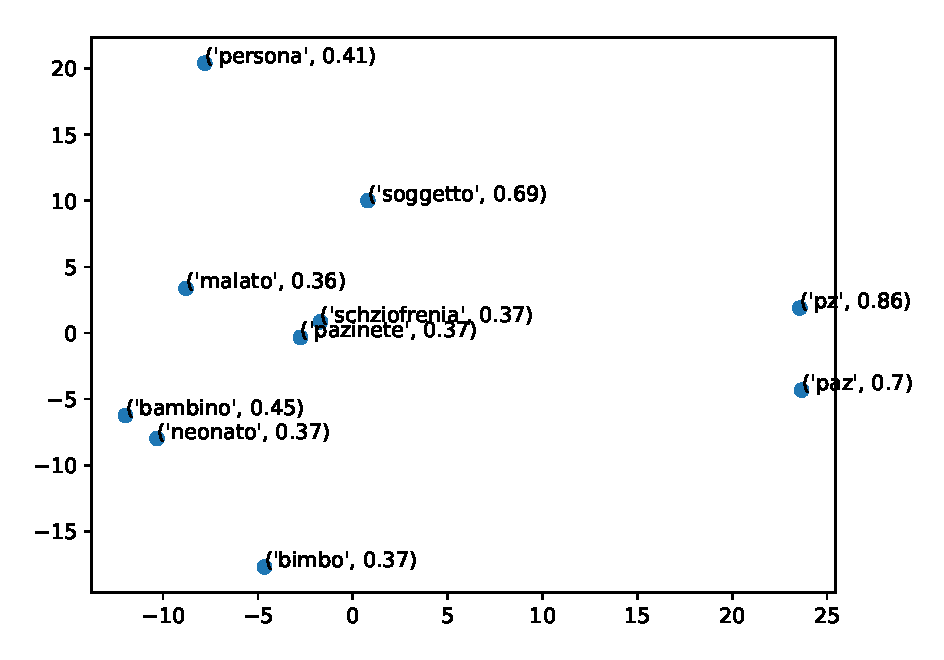
\includegraphics[width=.7\textwidth, height=.5\textheight, keepaspectratio]{pazienteJoinData}
	\caption[Patient - 10 most similar words plotted for JoinData model]{Top 10 most similar words to \textit{paziente} (patient) in the JoinData model.}
	\label{fig:pazienteJoinData}
\end{figure}


%Grafici delle TOp10


Figure \ref{fig:chartSDO} shows top ten most frequent words in the emergency room discharge records corpus. As we can see the words are: \textit{cardiopatia} (hearth disease), \textit{dolore} (pain), \textit{addominale} (abdomen), \textit{ipertensione} (hypertension), \textit{dx} (abbreviation of right), \textit{pz} (abbreviation of patient), \textit{diabete} (diabetes), \textit{paziente} (patient), \textit{trauma} (trauma) and \textit{cronica} (chronic).
The word \textit{cardiopatia} shows up \textbf{92'639} times (on \textbf{20'281'315} total words) in the diagnosis. \\
%TODO: explain why
According to data obtained under the \enquote*{CUORE} project\footnote{\url{http://www.salute.gov.it/imgs/C_17_navigazioneSecondariaRelazione_1_listaCapitoli_capitoliItemName_1_scarica.pdf}}, applying the incidence estimates on the population aged 35-74 years recorded by the Istat\footnote{\label{istat}Italian Statistic National Institute} 2001 Census, the number of new coronary events is around 80,000 per year in men and 20,000 per year for women.
In addition, the hearth diseases are placed, according to a study of Istat\footref{istat} on the first 25 causes of death in 2013-2014, among the top 3 causes of death in Italy.
\begin{figure}[ht]
	\centering
	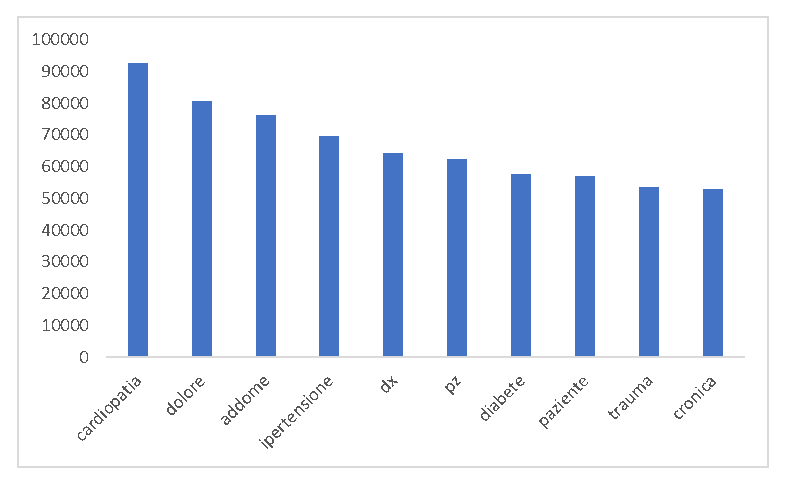
\includegraphics[width=.8\textwidth, height=.6\textheight, keepaspectratio]{chartSDO}
	\caption[Top 10 most frequent words in emergency room discharge records]{Top 10 most frequent words in the emergency room discharge records corpus.}
	\label{fig:chartSDO}
\end{figure}


Figure \ref{fig:chartWikipedia} shows top ten most frequent words in the Wikipedia health-related corpus. As we can see the words are: \textit{essere} (to be), \textit{altri} (others), \textit{viene} (comes), \textit{portale} (portal), \textit{consultato} (consulted), \textit{solo} (only), \textit{possono} (can), \textit{medicina} (medicine), \textit{parte} (part) and isbn\footnote{International Standard Book Number}.
The word \textit{essere} (to be) shows up \textbf{36484} times (on \textbf{13'195'758} total words) in the corpus data.\\
%TODO: explain why
This is a very common word in Wikipedia, placed among the top 62 in all Wikipedia rank.\footnote{\url{https://en.wiktionary.org/wiki/Wiktionary:Frequency_lists/Italian1000}} Indeed the word \textit{essere} (to be) shows 2'042 millions of times in all italian Wikipedia pages. One thing that is unpredictable in Wikipedia is that is not an official source of data, so basically it is up to who edits a Wikipedia page to write in his/her own style.\\
\begin{figure}[ht]
	\centering
	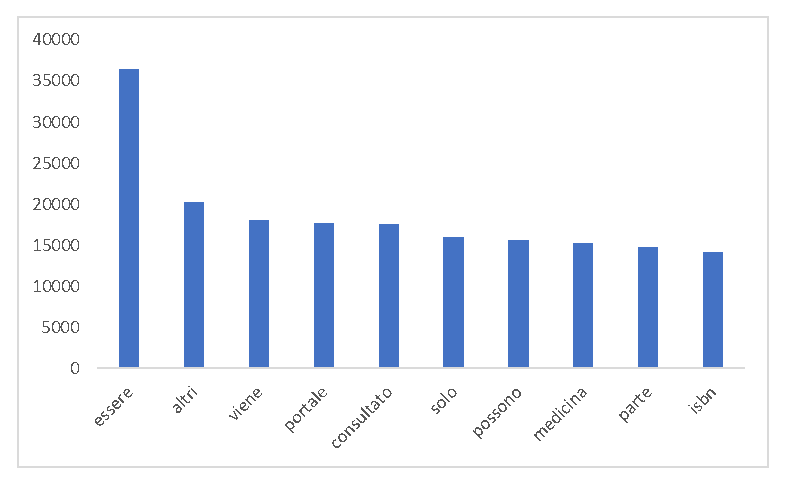
\includegraphics[width=.8\textwidth, height=.6\textheight, keepaspectratio]{chartWikipedia}
	\caption[Top 10 most frequent words in Wikipedia health-specific corpus]{Top 10 most frequent words in the Wikipedia health-related corpus.}
	\label{fig:chartWikipedia}
\end{figure}


Figure \ref{fig:chartDictionary} shows top ten most frequent words in the dictionary. As we can see the words are: \textit{altre} (other), \textit{specificata} (specified), \textit{senza} (without), \textit{menzione} (mention), \textit{frattura} (fracture),  \textit{perdita} (loss), \textit{tumori} (tumors), \textit{traumatismo} (traumas), \textit{coscienza} (consciousness) and \textit{condizione} (condition).
The word \textit{altre} (other) shows up \textbf{1761} times (on \textbf{130'218} total words) in the vocabulary.\\
%TODO: explain why
This is intuitively obvious, as ICD-9-CM contains more than 16 thousand classes while ICD-10-CM contains more than 60 thousands. Since even ICD-10-CM is not exhaustive, so many diseases will be specified under the category code that cites the word \textit{altre} (others) in the definition. Of course this still applies to ICD-9-CM that contains 1 on six specific definitions compared to ICD-10-CM.\\
Table \ref{tab:tableICd9CMaltre} shows first 5 coded diagnosis that contains the word \textit{altre} (others) in the definition's vocabulary.

\begin{table}[h!]
	\begin{center}  
		\caption[First 5 ICD-9-CM coded diagnosis that contains the word \textit{altre} (other)]{First 5 ICD-9-CM coded diagnosis that contains the word \textit{altre} (other) in the definition's vocabulary.} 
		\label{tab:tableICd9CMaltre}
		%\resizebox{\linewidth}{!}{  %
		\begin{tabular}{|p{\linewidth}|} 
			%\toprule
			%\textbf{Diagnosis} \\
			%\midrule
			\hline
			\textbf{003} - \textbf{Altre} infezioni da Salmonella	\\ \hline
			\textbf{00329} - \textbf{Altre} infezioni localizzate da Salmonella	\\ \hline
			\textbf{0038} - \textbf{Altre} infezioni specifiche da Salmonella	\\ \hline
			\textbf{0048} - \textbf{Altre} infezioni specifiche da Shigella	\\ \hline
			\textbf{005} - \textbf{Altre} intossicazioni alimentari (batteriche)	\\ \hline \hline
			\textbf{003} - \textbf{Other} salmonella infections	\\ \hline
			\textbf{00329} - Local salmonella inf NEC	\\ \hline
			\textbf{0038} - Salmonella infection NEC	\\ \hline
			\textbf{0048} - Shigella infection NEC \\ \hline
			\textbf{005} - \textbf{Other} food poisoning (bacterial)	\\ \hline
			%\bottomrule 
		\end{tabular} 
		%}
	\end{center}
\end{table}

\begin{figure}[ht]
	\centering
	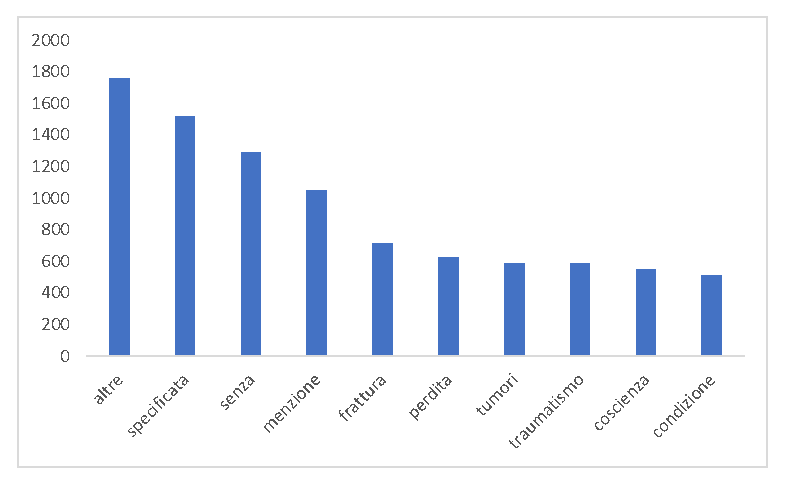
\includegraphics[width=.8\textwidth, height=.6\textheight, keepaspectratio]{chartDictionary}
	\caption[Top 10 most frequent words in ICD-9-CM Dictionary]{Top 10 most frequent words in the dictionary corpus.}
	\label{fig:chartDictionary}
\end{figure}


%Modelli prodotti e perchè ognuno contribuisce
We trained 4 models one for each corpus data and one joining all health-specific datasets calling it \enquote*{JoinData} model. Each corpus is essential to result in a complete health-specific word embeddings. 

This corpus data is essential for plenty of reasons. First of all, we have a lot of examples of how doctors write diagnosis and emergency room discharge records. Secondly we have all the medical jargon (or lingo) that in Italy, and especially in Forlì Hospital, doctors use. Moreover, we can take in consideration all the typo errors and common mistakes doctors often do when writing discharge records. Everything that is in this corpus is essential for the real approach to the diagnosis. 

This corpus is the most used corpus data for word embeddings. It's easy to download, there's no copyright issues and also it's available in almost every language you need. Downloading only the health-specific pages increased not only the quantity of words vectors in the word embedding but also the correct spelled medical words and some other non-doctors spoken terms that can be useful especially to those who aren't medical expert.

This corpus is essential for 2 main reasons: first it let us have the right terms and definition of each diagnosis and secondly we can have in the embeddings all the possible diagnosis, especially those who aren't likely to be found maybe because of Forlì Hospital isn't that big or because in Italy we haven't some diseases due to their rareness. 


Our main purpose is to show that domain-specific word embeddings is actually better than general word embedding trained with a big data corpus.\\As a matter of fact what we can show is trying to find out most similar words to health-related terms and see which words are more close to the meaning in each model. We expect that our \enquote*{JoinData} model that was trained with emergency room discharge records, wikipedia health-specific pages and the ICD-9-CM dictionary performs better than any other separate model and all of them performs better than a general model.\\
We choose to evaluate the word: \textit{arteria} (artery) and \textit{frattura} (fracture).\\
As we can see from table \ref{tab:tableTEDData} most similar words are awful results. Most certainly, the TED corpus data used to train the model didn't have medical terms or data.\\

\begin{table}[h!]
	\begin{center}
		\caption[General purpose - Most similar words in TED corpus model.]{Most-similar words to: \textit{arteria} (artery) and \textit{frattura} (frattura) in the TED corpus model.}
		\label{tab:tableTEDData}
		%\resizebox{\linewidth}{!}{  %
		\begin{tabular}{c|S|c|S}
			\toprule
			\textbf{Arteria} & \textbf{Value} & \textbf{Frattura} & \textbf{Value} \\
			\midrule
			l'omosessualità & 0.5719500184059143 & un'arteria & 0.5102593898773193 \\
			davanzale & 0.538368284702301 & difetto & 0.4904586970806122 \\
			indirizzano & 0.5319322943687439 & pretesto & 0.47922807931900024 \\
			l'interferenza & 0.5304628610610962 & turchese & 0.4672805964946747 \\			
			immutato	& 0.5259894132614136 & mina & 0.46371641755104065 \\
			\bottomrule
		\end{tabular}
		%}
	\end{center}
\end{table}

\begin{figure}[ht]
	\centering
	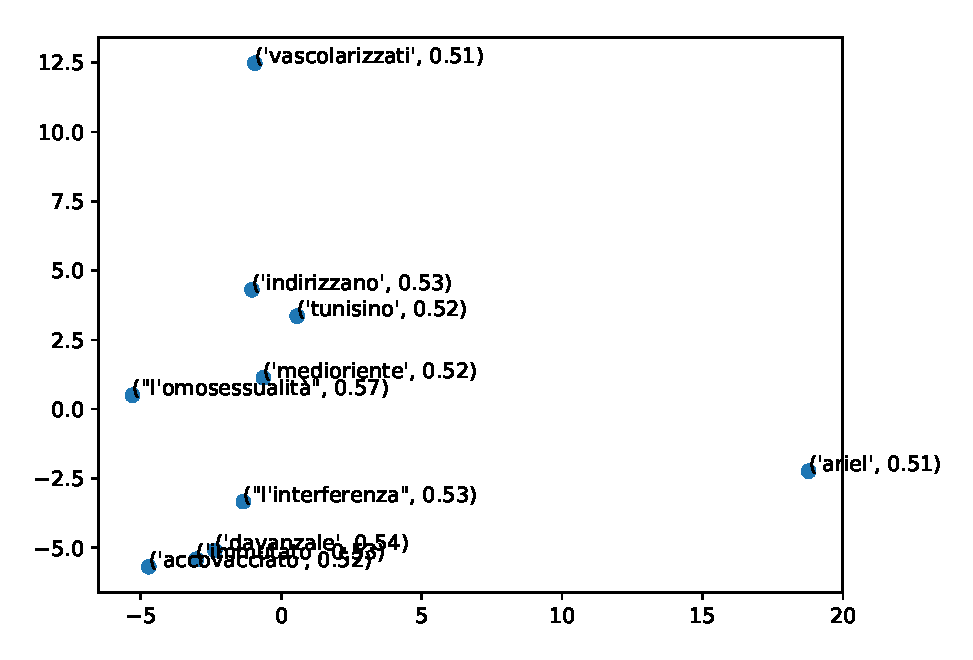
\includegraphics{arteriaTEDCorpus}
	\caption[Artery - 10 most similar words plotted for TED Corpus model]{Plotting 10 most similar word vectors to \textit{arteria} (artery) in the Ted Corpus model.}
	\label{fig:arteriaTEDCorpus}
\end{figure}

Table \ref{tab:tableWikipediaGeneralData} shows that wikipedia data are actually better than TED corpus. Wikipedia is often used for training word embeddings models and our corpus built with petscan and querying the wikimedia API is of course a subset of the general one. So we expect that table \ref{tab:tableWikipediaGeneralData} and table \ref{tab:tableWikipediaSpecific} perform with similar results. We can see this guess is true by the plotting of the word vectors of the top 10 most similar word to \textit{arteria} (artery) in figure \ref{fig:arteriaWikipediaGeneralCorpus} and \ref{fig:arteriaWikipediaSpecific}.

\begin{table}[h!]
	\begin{center}
		\caption[General purpose - Most similar words in Wikipedia corpus model]{Most-similar words to: \textit{arteria} (artery) and \textit{frattura} (frattura) in the general Wikipedia corpus model.}
		\label{tab:tableWikipediaGeneralData}
		%\resizebox{\linewidth}{!}{  %
		\begin{tabular}{c|S|c|S}
			\toprule
			\textbf{Arteria} & \textbf{Value} & \textbf{Frattura} & \textbf{Value} \\
			\midrule
			arterie & 0.8144235610961914 & clavicola & 0.7025632858276367 \\
			succlavia & 0.7115326523780823 & fratture & 0.6997483968734741 \\
			mesenterica & 0.7061030864715576 & perone & 0.6639930605888367 \\
			gastroepiploica & 0.7054485082626343 & lussazione & 0.6630574464797974 \\			
			l'arteria	& 0.7000836133956909 & rottura & 0.6615899801254272 \\
			\bottomrule
		\end{tabular}
		%}
	\end{center}
\end{table}

\begin{figure}[ht]
	\centering
	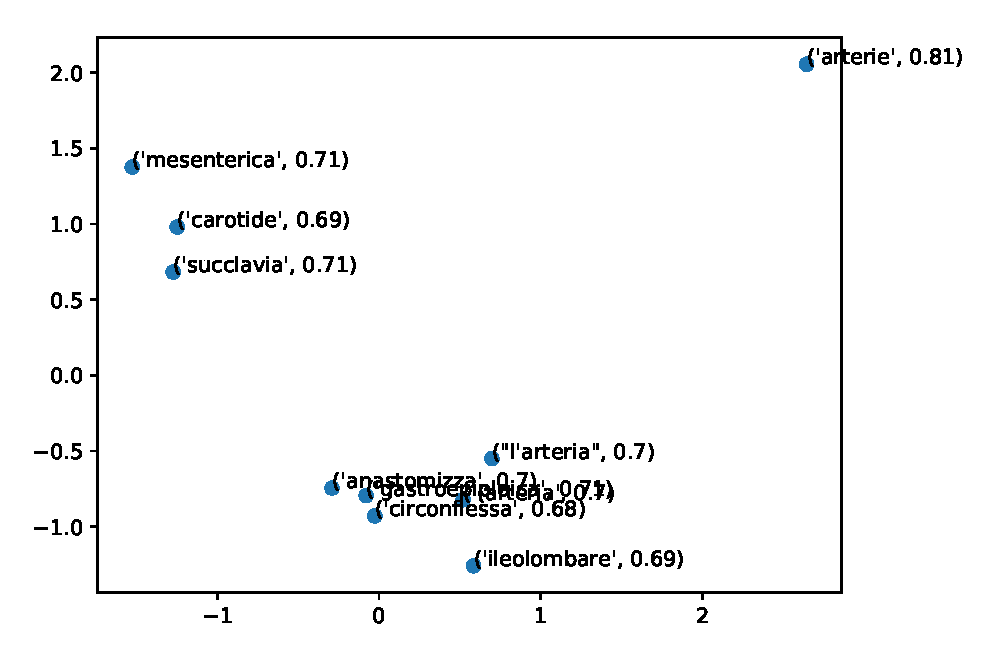
\includegraphics{arteriaWikipediaGeneral}
	\caption[Artery - 10 most similar words plotted for Wikipedia General Corpus model]{Plotting 10 most similar word vectors to \textit{arteria} (artery) in the general Wikipedia corpus model.}
	\label{fig:arteriaWikipediaGeneralCorpus}
\end{figure}

By comparing tables \ref{tab:tableTEDData} and \ref{tab:tableWikipediaGeneralData} with our best domain-specific model that shows its results in table \ref{tab:tableJoinData} we can confirm that domain-specific models are actually more precise than the general one.

\begin{table}[h!]
	\begin{center}
		\caption[Domain Specific - Most similar words in JoinData model]{Most-similar words to: \textit{arteria} (artery) and \textit{frattura} (frattura) in the JoinData model.}
		\label{tab:tableJoinData}
		%\resizebox{\linewidth}{!}{  %
		\begin{tabular}{c|S|c|S}
			\toprule
			\textbf{Arteria} & \textbf{Value} & \textbf{Frattura} & \textbf{Value} \\
			\midrule
			vena & 0.5782474279403687 & infrazione & 0.7564789056777954 \\
			artria & 0.536841630935669 & frattuta & 0.5775776505470276 \\
			ostio & 0.5062000751495361 & dolentefrattura & 0.5707343816757202 \\
			embolizzazione & 0.4836183786392212 & lussazion & 0.5554260015487671 \\			
			auricola	& 0.48101741075515747 & fratture & 0.5435724854469299 \\
			\bottomrule
		\end{tabular}
		%}
	\end{center}
\end{table}

\begin{figure}[ht]
	\centering
	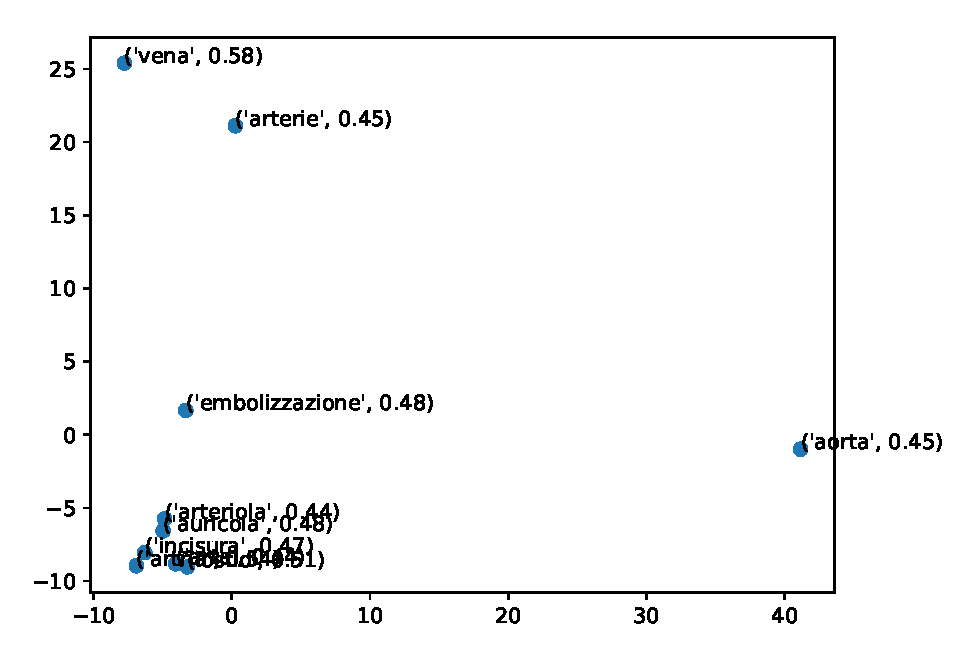
\includegraphics{arteriaJoinData}
	\caption[Artery - 10 most similar words plotted for JoinData model]{Plotting 10 most similar word vectors to \textit{arteria} (artery) in the JoinData model.}
	\label{fig:arteriaJoinData}
\end{figure}

Having a look at tables \ref{tab:tableSDO} and \ref{tab:tableDictionary} we can see how specific corpus word embeddings performs. As a matter of facts, we see that for the word embedding trained only with ICD-9-CM dictionary data, most-similar words are all medical terms that you can find in the official diagnosis provided by the italian Minister of Health. The first result \textit{carotide} (carotid artery) is actually the most important artery in our body.\\
For what concern the model trained with only emergency room discharge records, we expect unofficial medical terms, written in medical jargon or with typo errors. Indeed, the top result for artery is: \textit{artria} (typo error of artery), an evident typo of \textit{arteria} (artery). We can look at the top 10 most similar words vectors to \textit{artery} (artery) in Figure \ref{fig:arteriaSDO}.

\begin{table}[h!]
	\begin{center}
		\caption[Domain Specific - Most similar words in dictionary corpus model]{Most-similar words to: \textit{arteria} (artery) and \textit{frattura} (frattura) in the dictionary data model.}
		\label{tab:tableDictionary}
		%\resizebox{\linewidth}{!}{  %
		\begin{tabular}{c|S|c|S}
			\toprule
			\textbf{Arteria} & \textbf{Value} & \textbf{Frattura} & \textbf{Value} \\
			\midrule
			carotide & 0.9353908896446228 & base & 0.8839679956436157 \\
			vena & 0.8748384118080139 & chiusa & 0.8772594928741455 \\
			basilare & 0.8705806732177734 & volta & 0.8714847564697266 \\
			occlusione & 0.8691310882568359 & cranica & 0.865827202796936 \\
			aneurisma & 0.8563342094421387 & diafisi & 0.8557114005088806 \\
			\bottomrule
		\end{tabular}
		%}
	\end{center}
\end{table}

\begin{figure}[ht]
	\centering
	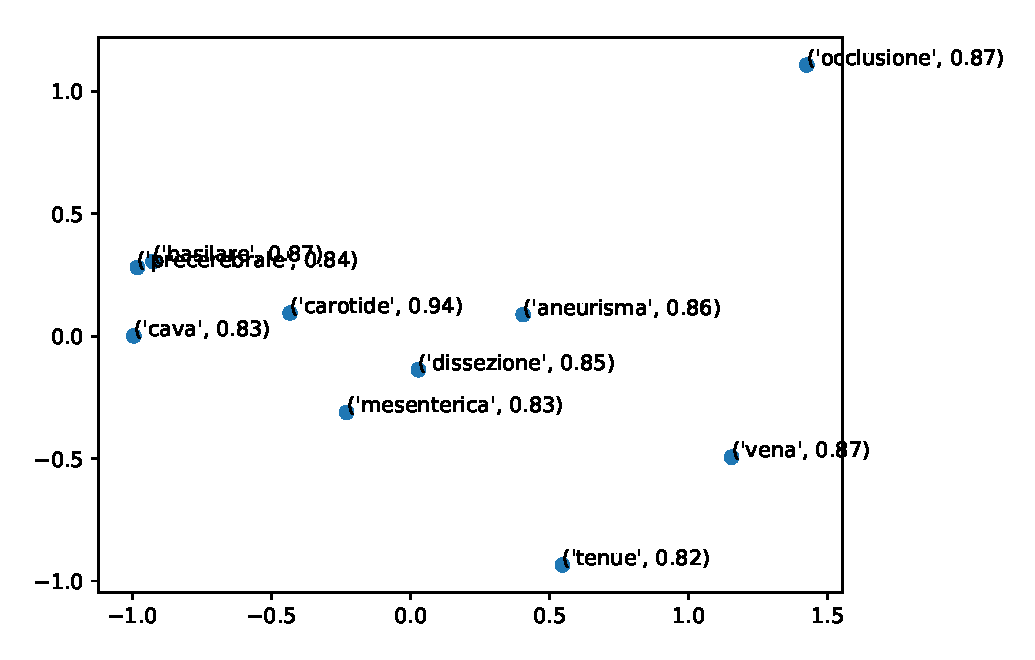
\includegraphics{arteriaDictionary}
	\caption[Artery - 10 most similar words plotted for dictionary corpus model]{Plotting 10 most similar word vectors to \textit{arteria} (artery) in the Dictionary data model.}
	\label{fig:arteriaDictionary}
\end{figure}

\begin{table}[h!]
	\begin{center}
		\caption[Domain Specific - Most similar words in Wikipedia health-specific corpus model]{Most-similar words to: \textit{arteria} (artery) and \textit{frattura} (frattura) in the Wikipedia health-specific corpus model.}
		\label{tab:tableWikipediaSpecific}
		%\resizebox{\linewidth}{!}{  %
		\begin{tabular}{c|S|c|S}
			\toprule
			\textbf{Arteria} & \textbf{Value} & \textbf{Frattura} & \textbf{Value} \\
			\midrule
			aorta & 0.6617274880409241 & tibia & 0.6638175249099731 \\
			vena & 0.6292352676391602 & lussazione & 0.6621222496032715 \\
			biforcazione & 0.6230939030647278 & deformazione & 0.6315639019012451 \\
			aneurisma & 0.5884683132171631 & deformità & 0.5965514779090881 \\
			uretere & 0.587216854095459 & fratture & 0.58837890625 \\
			\bottomrule
		\end{tabular}
		%}
	\end{center}
\end{table}

\begin{figure}[ht]
	\centering
	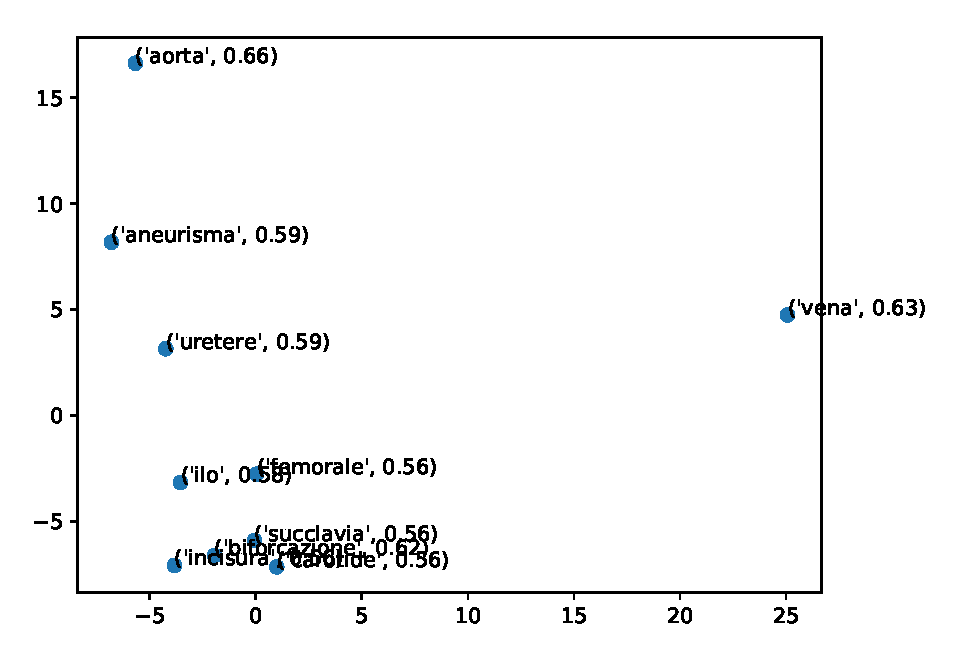
\includegraphics{arteriaWikipedia}
	\caption[Artery - 10 most similar words plotted for Wikipedia health-specific model]{Plotting 10 most similar word vectors to \textit{arteria} (artery) in the Wikipedia health-specific data model.}
	\label{fig:arteriaWikipediaSpecific}
\end{figure}

\begin{table}[h!]
	\begin{center}
		\caption[Domain Specific - Most similar words in emergency room discharge records corpus model]{Most-similar words to: \textit{arteria} (artery) and \textit{frattura} (frattura) in the emergency room discharge records corpus model.}
		\label{tab:tableSDO}
		%\resizebox{\linewidth}{!}{  %
		\begin{tabular}{c|S|c|S}
			\toprule
			\textbf{Arteria} & \textbf{Value} & \textbf{Frattura} & \textbf{Value} \\
			\midrule
			artria & 0.5504277944564819 & infrazione & 0.7562589049339294 \\
			ostio & 0.5062978863716125 & fratture & 0.4931909143924713 \\
			auricola & 0.49559450149536133 & frattuta & 0.4765438437461853 \\
			comune & 0.47281068563461304 & aafrattura & 0.4575194716453552 \\
			pta & 0.47225064039230347 & fratura & 0.4515219032764435 \\
			\bottomrule
		\end{tabular}
		%}
	\end{center}
\end{table}

\begin{figure}[ht]
	\centering
	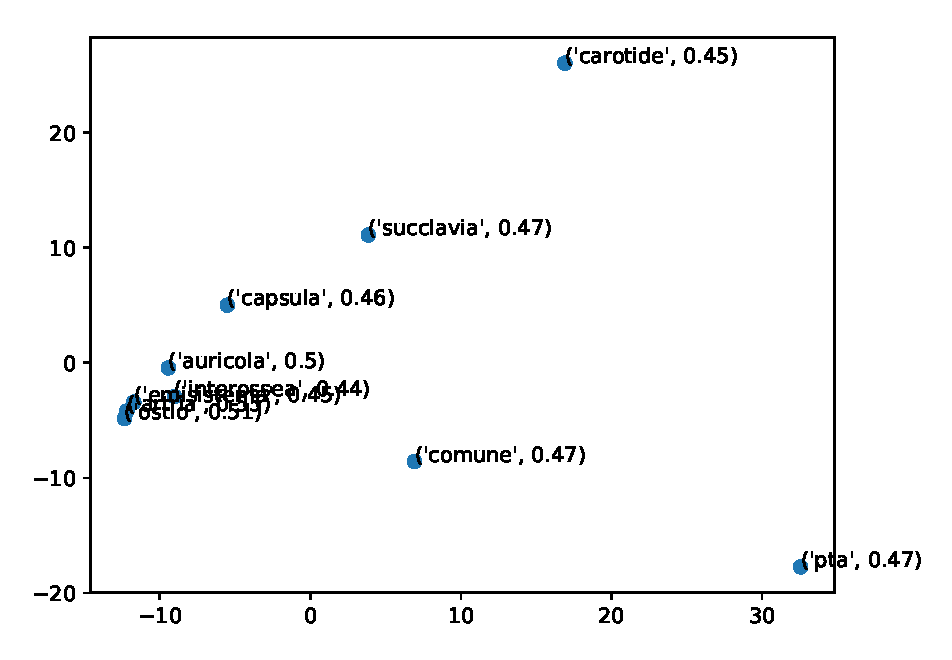
\includegraphics{arteriaSDO}
	\caption[Artery - 10 most similar words plotted for Emergency room discharge records model]{Plotting 10 most similar word vectors to \textit{arteria} (artery) in the emergency room discharge records corpus model.}
	\label{fig:arteriaSDO}
\end{figure}



In a related work, we tried to automatically assign the codes corresponding to a textual diagnosis through a classifier. This classifier used our domain-specific word embedding for weighting words instead of using a general-purpose one and noticed a real gain in terms of accuracy.


This supervised classifier was trained using a 14-thousands-diagnosis dataset (that is just a tiny subset of the more than 700 thousands diagnosis collected from Forlì emergency room) manually labeled by qualified personnel.\\
Textual diagnoses were first preprocessed in order to minimize spelling errors and meaningless symbols. In this process, we built a token dictionary of words contained in the training set.\\
Subsequently we created an embedding matrix where multidimensional vector were associated to each word of each diagnosis.
To build the embedding matrix we start from a matrix of dimension = (number of words in the diagnosis, length of the embedding vector) where each element is initialized to 0. The matrix is progressively filled by iterating on the tokenizer indexes, where each row corresponds to an index(and therefore to a corresponding word) and its content is the word vector embedded.
This embedding matrix is used to associate a certain weight with words of the input diagnosis to the classifier in order to capture the semantics of sentences and increase final precision.



We computed the accuracy of each word embedding through the f1 score\footnote{\url{http://scikit-learn.org/stable/modules/generated/sklearn.metrics.f1_score.html}} of the built classifier. The F1 score can be interpreted as a weighted average of the precision and recall, where an F1 score reaches its best value at 1 and worst score at 0. The relative contribution of precision and recall to the F1 score are equal.\\The formula for the F1 score is:\\
\begin{lstlisting}
F1 = 2 * (precision * recall) / (precision + recall)
\end{lstlisting}
where:
\begin{itemize}
	\item \textbf{Precision:} is the fraction of relevant instances among the retrieved instances.
	\item \textbf{Recall:} is the fraction of relevant instances that have been retrieved over the total amount of relevant instances.
\end{itemize}
We can see in table \ref{tab:tableF1Micro} results of F1 micro\footnote{Calculate metrics globally by counting the total true positives, false negatives and false positives.} and table \ref{tab:tableF1Weighted} shows the results of F1 weighted\footnote{Calculate metrics for each label, and find their average weighted by support (the number of true instances for each label). This alters ‘macro’ to account for label imbalance; it can result in an F-score that is not between precision and recall.}.
\begin{table}[h!]
	\begin{center}
		\caption[F1 Micro of each word embedding, both domain-specific and general purpose]{F1 Micro of each word embedding, both domain-specific and general purpose}
		\label{tab:tableF1Micro}
		%\resizebox{\linewidth}{!}{  %
		\begin{tabular}{l|S}
			\toprule
			\textbf{Word embeddings} & \textbf{Value} \\
			\midrule
			\textbf{JoinData} & \textbf{0.18}  \\
			Emergency room discharge records & 0.17 \\
			Wikipedia health-specific & 0.11  \\
			Wikipedia general & 0.05 \\
			Dictionary ICD-9-CM & 0.04  \\
			TED corpus & 0.04  \\
			\bottomrule
		\end{tabular}
		%}
	\end{center}
\end{table}

\begin{table}[h!]
	\begin{center}
		\caption[F1 Weighted of each word embedding, both domain-specific and general purpose]{F1 Weighted of each word embedding, both domain-specific and general purpose}
		\label{tab:tableF1Weighted}
		%\resizebox{\linewidth}{!}{  %
		\begin{tabular}{l|S}
			\toprule
			\textbf{Word embeddings} & \textbf{Value} \\
			\midrule
			\textbf{JoinData} & \textbf{0.233}  \\
			Emergency room discharge records & 0.210 \\
			Wikipedia health-specific & 0.175  \\
			Wikipedia general & 0.129 \\
			TED corpus & 0.106  \\
			Dictionary ICD-9-CM & 0.105  \\
			\bottomrule
		\end{tabular}
		%}
	\end{center}
\end{table}

As we can clearly see from this results, we can conclude that domain-specific word embeddings is more suitable for this task. Moreover the JoinData model is undoubtedly the most accurate among the other word embeddings, mostly over the general purpose word embeddings.